67. \begin{figure}[ht!]
\center{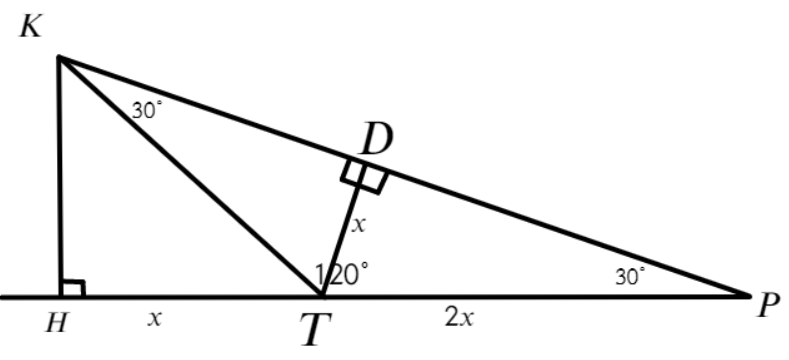
\includegraphics[scale=0.35]{g67.png}}
\end{figure}\\
Чтобы найти расстояние от $T$ до $PK,$ проведём $TD\perp PK.$ Найдём $\angle P=180^\circ-120^\circ-30^\circ=30^\circ,\ \angle KTD=90^\circ-30^\circ=60^\circ, \angle KTH=180^\circ-120^\circ=60^\circ.$ Тогда прямоугольные треугольники $KTD$ и $KTH$ равны по гипотенузе ($KT$ --- общая) и острому углу, а значит $TD=TH.$ Обозначим $TD=x,$ тогда по теореме о катете, лежащем напротив угла в $30^\circ$ для треугольника $TDP,$ имеем $TP=2x.$ Таким образом, $HP=TH+TP=x+2x=3x=21$см, откуда $TD=x=7$см.\\
